\title{Mapeamento Digital no Ensino de Ciência do Solo}
\subtitle{Capacitação e Perspectivas para o Futuro do Levantamento de Solos no País}
\author{por Helena Saraiva Koenow Pinheiro}
\maketitle
\begin{wrapfigure}{l}{0.15\textwidth}
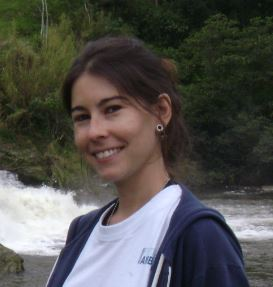
\includegraphics[width=0.15\textwidth]{figuras/helena}
\end{wrapfigure}
O mapeamento de solos enfrenta nos dias de hoje grandes desafios para atender a demanda da sociedade por informações em nível de detalhe adequado para o planejamento de uso da terra e dos recursos naturais. Paralelamente, a melhoria da capacidade de processamento dos computadores aliada a disponibilidade de programas e dados estruturados em ambiente de Sistemas de Informações Geográficas (SIG), impulsiona a utilização de novas ferramentas e métodos de análise aplicados aos estudos ambientais.\\
A formação de novos pedólogos vivência um momento emblemático, que pode ser considerado um hiato no contexto do levantamento de solos no país, onde se denota carência em transferência de conhecimentos e experiências práticas, agravada pela ausência de grandes projetos e incentivos governamentais para treinamento e capacitação deste tipo de profissional, diga-se de passagem, escasso no país.\\
Neste contexto, o ensino de ciências do solo reflete a necessidade de atualização e discussão de conceitos e métodos clássicos, considerando a inserção de ferramentas modernas de análise espacial buscando aperfeiçoar os procedimentos inerentes à atividade de levantamento, desde o planejamento amostral até a análise e apresentação dos dados obtidos. Não obstante, o uso de técnicas de Mapeamento Digital de Solos (MDS) confere um caráter quantitativo, com conhecimento das incertezas associadas aos produtos gerados, tendo como base procedimentos estatísticos reproduzíveis, conforme apresentado por \cite{CarvalhoJuniorEtAl:2011, ChagasEtAl:2011, CrivelentiEtAl:2009, GiassonEtAl:2006, WiesmeierEtAl:2010, tenCatenEtAl:2011}.\\
A oportunidade de participar de uma disciplina direcionada ao MDS motivou a elaboração deste artigo, que tem o objetivo principal de relatar a experiência como aluna de doutorado do Curso de Pós-Graduação em Agronomia -- Ciência do Solo (CPGA-CS, UFRRJ), membro integrante da Rede Brasileira de Pesquisa em Mapeamento Digital de Solos (RedeMDS) e da Comissão de Pedometria da Sociedade Brasileira de Ciência do Solo (Divisão 1.3.1 da SBCS).\\
Em primeira instância, encarei esta oportunidade como uma forma de contribuir para a discussão dos procedimentos intrínsecos ao levantamento de solos, relevantes para a formação de novos pedólogos e consequentemente, para a continuidade e prosperidade desta nobre profissão, restrita à experiência e conhecimento tácito de alguns profissionais, cada vez mais raros. Dito isso, escrevo este artigo para prestigiar a iniciativa de difusão do conhecimento nesta temática considerada pioneira no país, no que tange ao ensino e capacitação de novos pedólogos no uso de ferramentas modernas de análise espacial de dados e mapeamento digital.\\
A disciplina intitulada ``Métodos e Técnicas de Mapeamento Digital de Solos (Tópicos Especiais em Ciência do Solo-T.E.C.S.)'', oferecida no Curso de Pós-Graduação em Agronomia - Ciência do Solo (CPGA-CS), teve como público alvo estudantes de pós-graduação e professores da Universidade Federal Rural do Rio de Janeiro (UFRRJ).\\
De uma forma geral, as aulas ministradas abordaram o manuseio de dados primários e obtenção de secundários, treinamento com ferramentas de SIG e programas específicos, formas de aplicação e análise de modelos preditivos no mapeamento de classes e atributos dos solos.\\
O período de duração da disciplina coincidiu com a realização da 3º Reunião da RedeMDS e do 34º Congresso Brasileiro de Ciência do Solo (XXXVI CBCS), no mês de agosto na cidade de Florianópolis (SC) que promoveu o encontro de pesquisadores e estudantes para discussão de assuntos relacionados a esta temática.\\
Este conjunto de circunstâncias contou ainda com uma feliz coincidência que merece ser mencionada no contexto desta narrativa. Após o término dos eventos supracitados a UFRRJ recebeu a visita do pesquisador Philip Owens, Professor da Universidade de Purdue (Indiana - EUA). Tal fato oportuno ocorreu no período de aulas da disciplina, o que propiciou o contato e a troca de experiências com professor de instituição estrangeira de excelência no ensino de ciências agrárias, com potencial para construção de parceria e intercâmbio de estudantes e pesquisadores. Philip prestou contribuição à disciplina na forma de palestras, onde expôs parte das suas ideias e trabalhos relacionados ao emprego de MDS na hidropedologia, mostrando uma gama de possibilidades para aquisição de dados e de interpretação dos produtos derivados dos levantamentos de solos. E ainda, ressaltou que o uso destas técnicas tem em vista fornecer informações úteis e estratégicas para a sociedade que sirvam como subsídio para o planejamento de uso dos 
recursos naturais. Em suas explanações preconizou a aplicação destas técnicas na avaliação do potencial e das limitações das terras para produção agrícola entre outras atividades, destacando a importância do solo como organismo natural atuante na renovação (filtragem da água), recarga, conservação e manutenção de mananciais hídricos superficiais e sub-superficiais.\\
Sendo assim, a difusão de técnicas e capacitação de profissionais no uso das ferramentas e análise de dados em ambiente SIG, tem cunho estratégico e promissor contribuindo para o desenvolvimento científico e inovação tecnológica do país. Não obstante, as informações que podem ser extraído vão além da representação espacial de dados de solos, servido de base para estudos relacionados à prospecção mineral, dinâmica da água, potencial agrícola, aspectos geotécnicos, entre outras interpretações. Sob a ótica da taxonomia e classificação de solos é possível que a aplicação extensiva destas técnicas possa facilitar a identificação de fatores locais típicos para definição de classes em nível categórico de famílias e series, possibilitando o estudo da variabilidade das propriedades das distintas classes de solos e níveis categóricos.\\
Acredito em um ``futuro não muito distante'' onde a importância do MDS seja reconhecida e difundida através de criação de linha de pesquisa com enfoque em pedometria e mapeamento, com inserção de disciplinas regulares que abordem esta temática na formação de novos pedólogos. Sob um ponto de vista mais abrangente, ações desta natureza contribuem para melhor entendimento das relações solo-paisagem e aspectos do ambiente. Com o emprego extensivo de ferramentas e programas de geoprocessamento em estudos ambientais é plausível considerar que pesquisas estruturadas sob a perspectiva do MDS produzam ricos banco de dados georreferenciados e sistematizados, que são muito úteis para elaboração de modelos preditivos complexos e importantes para o planejamento de ocupação das terras e tomada de decisões relacionadas ao uso de recursos naturais.\\
Na primeira aula do curso foi indagado aos alunos quais as perspectivas individuais sobre a disciplina e as formas de aplicação das técnicas de MDS em seus respectivos estudos. Observei que inicialmente muitos dos participantes não imaginavam as possibilidades e diversidade de análises e interpretações dos produtos gerados. Este quadro se transformou com o passar das aulas, onde foi possível perceber o crescente interesse, através do surgimento de dúvidas e observações emitidas pelos participantes de forma direcionada às aplicações práticas do conhecimento adquirido.\\
Pessoalmente, tive a impressão que alguns dos participantes não tinham contato prévio com os softwares e técnicas utilizadas, sendo a familiarização com a linguagem e ambientação com os comandos e operações, construída gradativamente.\\
O treinamento preliminar em ferramentas e programas de geoprocessamento, e também o domínio dos conceitos de gênese de solos, modelos clássicos e padrões de ocorrência na paisagem e procedimentos do mapeamento, representaram fonte de complicação por parte de alguns alunos. Sendo assim, tais requisitos são desejáveis para melhor aproveitamento do conteúdo lecionado. Considero ainda, a subdivisão dos assuntos tratados na disciplina em dois âmbitos elementares, que podem ser objeto de módulos sequenciais. Um deles com caráter introdutório e abordagem teórica pode tratar dos conceitos básicos envolvidos na atividade de levantamento de solos, e procedimentos de pré-processamento e manuseio de dados espaciais georreferenciados, para obtenção das variáveis discriminantes e análise das co-relações solo-paisagem. O outro módulo tange ao treinamento em ferramentas de modelagem digital e algoritmos preditivos para o mapeamento digital de classes e atributos dos solos, incluindo a análise dos produtos do MDS, incertezas 
associadas e interpretações derivadas. O conteúdo deste módulo pode ser ministrado com base em um estudo de caso (dados reais), motivando a utilização destas técnicas em áreas de referência.\\
Diante do exposto, novamente parabenizo a concretização desta disciplina, que mesmo em caráter incipiente, como matéria de tópicos especiais oferecida para alunos pós-graduação, significa uma nova tendência no ensino de ciência de solo e inspira uma nova geração de pedólogos, com capacidade de compreensão e aplicação de conceitos clássicos e capacitação em ferramentas modernas de análise espacial, que possam contribuir com o aperfeiçoamento e retomada das atividades ligadas ao levantamento de solos no Brasil.\\
Cabe suscitar ainda, que a concretização do curso teve como precursora a existência da RedeMDS que promoveu a integração entre os pesquisadores deste ramo do conhecimento, o que inclui os responsáveis pela viabilização da disciplina e alguns alunos que utilizam MDS em seus estudos.\\
Enfim, espero que este relato sirva como incentivo e inspiração para estudantes, professores, técnicos, pesquisadores e instituições ligadas ao ensino de ciência do solo e capacitação de recursos humanos, para a difusão do conhecimento, possibilidades e limitações do uso de ferramentas de mapeamento digital aplicadas a levantamentos pedológicos.
\begin{footnotesize}
\begin{thebibliography}{99}
\bibitem[Carvalho Júnior et~al. (2003) Carvalho Júnior, Chagas, Fernandes, Vieira, Schaefer, Bhering, Francelino]{CarvalhoJuniorEtAl:2011}
W. de Carvalho Júnior, C. da S. Chagas, E.I. Fernandes, C.E. Vieira, C.E.G. Schaefer, S.B. Bhering, M.R. Francelino (2011)
\newblock Digital soilscape mapping of tropical hillslope areas by neural networks.
\newblock {\em Scientia Agricola} 68: 691-696.
\bibitem[Chagas et~al. (2011) Chagas, Carvalho Júnior, Bhering]{ChagasEtAl:2011}
C. de S. Chagas, W. de Carvalho Júnior, S.B. Bhering (2011)
\newblock Integração de dados do Quickbird e atributos do terreno no mapeamento digital de solos por redes neurais artificiais.
\newblock {\em R. Bras. Ci. Solo} 35: 693-704.
\bibitem[Crivelenti et~al. (2009) Crivelenti, Coelho, Adami, Oliveira]{CrivelentiEtAl:2009}
R.C. Crivelenti, R.M. Coelho, S.F. Adami, S.R. de M. Oliveira (2009)
\newblock Mineração de dados para a inferência de relações solo-paisagem em mapeamentos digitais de solo.
\newblock {\em Rev. Agro. Bras.} 44: 1707-1715.
\bibitem[Giasson et~al. (2006) Giasson, Clarke, Inda Junior, Merten, Tornquist]{GiassonEtAl:2006}
E. Giasson, R.T. Clarke, A.V. Inda Junior, G.H. Merten, C.G. Tornquist (2006)
\newblock Digital soil mapping using multiple logistic regression on terrain parameters in southern Brazil.
\newblock {\em Sci. Agric.} 63: 262-268.
\bibitem[ten Caten et~al. (2011) ten Caten, Dalmolin, Pedron, Mendonça-Santos]{tenCatenEtAl:2011}
A. ten Caten, R.S.D. Dalmolin, F.A. Pedron, M.L. Mendonça-Santos (2011)
\newblock Extrapolação das relações solo-paisagem a partir de uma área de referência.
\newblock {\em Ci. Rural.} 41: 812-816.
\bibitem[Wiesmeier et~al. (2010) Wiesmeier, Barthold, Blank,  Kögel-Knabner]{WiesmeierEtAl:2010}
M. Wiesmeier, F. Barthold, B. Blank,  I. Kögel-Knabner (2010)
\newblock Digital mapping of soil organic matter stocks using Random Forest modeling in a emi-arid steppe ecosystem.
\newblock {\em Plant Soil} 340: 7-24.
\end{thebibliography}
\end{footnotesize}
\address{Helena Saraiva Koenow Pinheiro\\
  Universidade Federal Rural do Rio de Janeiro\\
  \email{lenask@gmail.com}}